\section{Wahrscheinlichkeitsverteilung}

\subsection{Verteilungsfunktion}
\begin{minipage}{0.6\textwidth}
	\begin{tabular}{|l|l|l|}
		\hline
		\textbf{allgemein} & \textbf{diskret} & \textbf{kontinuierlich}\\
		\hline
		\hline
		$P(X\leq x)=F(x)$ & $=\sum\limits_{k=-\infty}^x p_k$ &
		$=\int\limits_{-\infty}^x \varphi(\tilde{x})d\tilde{x}$\\
		
		$P(X>x)=1-P(X\leq x)$ & & \\        	
		$P(a \le X < b)=F(b)-F(a)$ & $=\sum\limits_{k=a}^b p_k$ &
		$=\int \limits_a^b \varphi(\tilde{x})d\tilde{x}$\\
		\hline
	\end{tabular}
\end{minipage}
\begin{minipage}{0.4\textwidth}
	%Autor: Simon Walker
%Version: 1.0
%Datum: 09.12.2019
%Lizenz: CC BY-NC-SA

\begin{tikzpicture}[xscale=0.4, yscale=2.5]
	\def\xMin{-20}
	\def\xMax{20}
	\def\yValues{{0, 0, 0.00016, 0.00034, 0.00069, 0.00135, 0.00256, 0.00466, 0.0082, 0.0139, 0.02275, 0.03593, 0.0548, 0.08076, 0.11507, 0.15866, 0.21186, 0.27425, 0.34458, 0.42074, 0.5, 0.57926, 0.65542, 0.72575, 0.78814, 0.84134, 0.88493, 0.91924, 0.9452, 0.96407, 0.97725, 0.9861, 0.9918, 0.99534, 0.99744, 0.99865, 0.99931, 0.99966, 0.99984, 0.99993, 0.99997}}
	
	%Achse
	\draw[very thick, ->] (-8-0.5, 0) -- (8+0.5, 0);
	\draw[very thick, ->] (0, 0) -- (0, 1.2);
	\draw[dashed] (-8, 1) -- (8, 1);
	\node[above left] at (0, 1) {$1$};
	\node[right] at (\xMax+0.5, 0) {$x$};
	\node[above] at (0, 1.2) {W'keit $F(x)$};
	
	\draw[blue, very thick, smooth cycle]
	\foreach \i in {0, 1, ..., 39}{
		 ({(\xMin+\i)*0.4},  \yValues[\i]) -- ({(\xMin+\i+1)*0.4}, {\yValues[\i+1]})
	};
	
\end{tikzpicture}
\\
	Verteilungsfunktion der Normalverteilung
\end{minipage}


\subsubsection{Eigenschaften}
Bei einem Sprung gilt: \textbf{Sprunghöhe = Wahrscheinlichkeit des Wertes x}\\
$$\underbrace{\boxed{\mathbb{D}(F) = \mathbb{R}}}_{\text{Definitionsbereich}} \qquad \underbrace{\boxed{\mathbb{W}(F) \in[0,1]}}_{\text{Wertebereich}} \qquad \boxed{F(-\infty)=0} \qquad  \boxed{F(\infty)=1}
\qquad \boxed{F(x) \text{ ist monoton steigend}}$$

\hrule

\subsection{Wahrscheinlichkeitsdichte}
\begin{multicols}{2}
\textbf{Dichtefunktion oder Wahrscheinlichkeitsdichte:} \\
$\varphi(x) = F'(x)$ \\
\textbf{Bei Sprungstellen von F(x):} \\
$\varphi(x) = $ Dirac mit Gewichtung der Sprunghöhe\\
\textbf{Allgemein gilt:}\\
$\int\limits_{-\infty}^{\infty}\varphi (x) dx = 1$\\[1pt]

\textbf{Erwartungswert:} Wert mal W'keit\\
\begin{tabular}{l l l}
	$E(\textcolor{red}{X})$ &  
$ = \int\limits_{-\infty}^{\infty} \textcolor{red}{x} \cdot \varphi(x) dx$  & 
bzw. $\sum\limits_{-\infty}^{\infty} \textcolor{red}{x} \cdot p_k$\\

	$E(\textcolor{red}{X^2})$ & 
$ = \int\limits_{-\infty}^{\infty} \textcolor{red}{x^2} \cdot \varphi(x) dx$ & 
bzw. $\sum\limits_{-\infty}^{\infty} \textcolor{red}{x^2} \cdot p_k$\\

	$E(\textcolor{red}{X^N})$ & 
$ = \int\limits_{-\infty}^{\infty} \textcolor{red}{x^N} \cdot \varphi(x) dx$ 
& bzw. $\sum\limits_{-\infty}^{\infty} \textcolor{red}{x^N} \cdot p_k$
\end{tabular}

\columnbreak
%Autor: Simon Walker
%Version: 1.0
%Datum: 09.12.2019
%Lizenz: CC BY-NC-SA

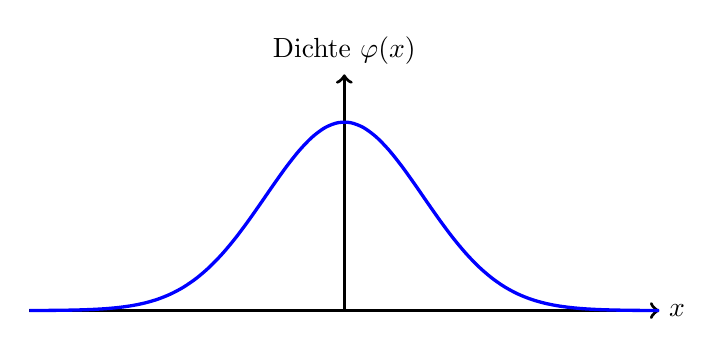
\begin{tikzpicture}[xscale=1, yscale=6]
	
	%Achse
	\draw[very thick, ->] (-4, 0) -- (4, 0);
	\draw[very thick, ->] (0, 0) -- (0, 0.5);
	\node[right] at (4, 0) {$x$};
	\node[above] at (0, 0.5) {Dichte $\varphi(x)$};
	
	\draw[blue, very thick, smooth]
	plot[smooth, samples=50, variable=\x, domain=-4:4]
		(\x, {0.3989*exp(-((\x)^2)/2)});

\end{tikzpicture}
\\
Wahrscheinlichkeitsdichte der Normalverteilung
\end{multicols}

\hrule


\subsection{Rechenregeln für $\varphi$ und $F$}
\begin{minipage}{11cm}
	\begin{tabular}{ll}
      	\textbf{Gegeben:} &X, Y Zufallsvariablen und $\varphi_X$, $\varphi_Y$
      	bekannt\\
   	\end{tabular}

   	\begin{tabular}{p{6cm}p{6cm}}
		\textbf{Verteilungsfunktion:} & \textbf{Dichte:}\\
		$F_{X+a}(x)=F_X(x-a)$  &$\varphi_{X+a}(x)=\varphi_X(x-a)$\\
		$F_{\lambda X}(x)=F_X(\frac{x}{\lambda})$ &$\varphi_{\lambda
		X}(x)=\varphi_X(\frac{x}{\lambda})\frac{1}{\lambda}$\\
		$F_{X+Y}(x)=F_X\ast\varphi_Y(y)=F_Y\ast\varphi_X(x)$ &
		$\varphi_{X+Y}(x)=\varphi_X\ast\varphi_Y(x)$\\
		$F_{\sqrt{X}}(x)=F_X(x^2)$ &
		$\varphi_{\sqrt{X}}(x)=2x\varphi_X(x^2)$\\
		$F_{X^2}(x)=F_X(\sqrt{x})-F_X(-\sqrt{x})$ &
		$\varphi_{X^2}(x)=\frac{1}{2}x^{-\frac{1}{2}}(\varphi_X(\sqrt{x})+\varphi_X(-\sqrt{x}))$
   	\end{tabular}
\end{minipage}
\begin{minipage}{7cm}
   	\subsubsection{Algorithmus Bsp.}
   	\begin{tabular}{ll}
		1. Definition von $F$ anwenden: $F_{\lambda X}(x)=P(\underbrace
		{\lambda X\leq x}_{*})$\\ 
		2. Bedingung * umformen: $P(X \leq
		\frac{x}{\lambda})=F_X(\frac{x}{\lambda})$\\ 
		3. für Dichte: $\frac{d}{dx}$\\
		\vspace{3mm}
		$\varphi_{\lambda X}(x)=\frac{d}{dx}F_{\lambda
		X}(x)=\frac{d}{dx}F_X(\frac{x}{\lambda})=
		\varphi_X(\frac{x}{\lambda})\frac{1}{\lambda}$
   	\end{tabular}
	\vspace{10mm}
\end{minipage}

\begin{multicols}{2}    
  \subsubsection{Maximalwert eines Intervalls}
    $X_1,\ldots X_i$ sind auf dem Intervall $[0,l]$ mit $F_X(x)$ verteilt\\
    M=$\max \{ X_1,\ldots,X_i\} $ \\
    $F_M(x)=F_X(x)^n$ \\
	\columnbreak
  \subsubsection{Median \skript{\pageref{sk-subsubsection-median}}}
    Der Median $med(X)$ von $X$ ist eine Zufallsvariable, welche für
    $F(med(X)) = \frac{1}{2}$ ist.
  
\end{multicols}

%\hrule

\subsection{Normalverteilung}
\begin{minipage}{10cm}
	Viele kleine, unabhängige Zufallsvariable sammeln sich zu einer
	normalverteilten Zufallsvariable.\\
	$\varphi(x)=\frac{1}{\sqrt{2
			\pi}\sigma}\cdot e^{-\frac{(x-\mu)^2}{2\sigma^2}} = N(\mu ; \sigma) $\\ 
	$F(x)=\frac{1}{\sqrt{2\pi}\sigma}\cdot \int\limits^{x}_{-\infty}{e^{-\frac{(\tilde{x} -\mu)^2}{2\sigma^2}}} d\tilde{x} $ \\
	Addieren von Normalverteilungen: \\
	\fbox{$N(\mu_{1} ; \sigma_{1}) + N(\mu_{2} ; \sigma_{2})
		= N(\mu_{1} + \mu_{2} ; \sqrt{\sigma_{1}^{2} + \sigma_{2}^{2}})$} \\
	Für $F(-x)$ gilt $F(-x) = 1 - F(x)$
\end{minipage}
\begin{minipage}{8cm}
	%Autor: Simon Walker
%Version: 1.0
%Datum: 09.12.2019
%Lizenz: CC BY-NC-SA

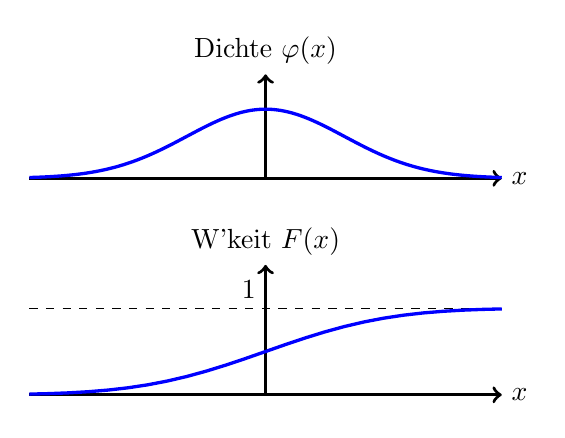
\begin{tikzpicture}[xscale=1, yscale=1.1]
	
	%Achse
	\draw[very thick, ->] (-3, 2.5) -- (3, 2.5);
	\draw[very thick, ->] (0, 2.5) -- (0, 3.7);
	\node[right] at (3, 2.5) {$x$};
	\node[above] at (0, 3.7) {Dichte $\varphi(x)$};
	
	\draw[blue, very thick, smooth]
	plot[smooth, samples=50, variable=\x, domain=-3:3]
		(\x, {2*0.3989*exp(-((\x)^2)/2) + 2.5});
		
	%Achse
	\draw[very thick, ->] (-3, 0) -- (3, 0);
	\draw[very thick, ->] (0, 0) -- (0, 1.5);
	\node[right] at (3, 0) {$x$};
	\node[above] at (0, 1.5) {W'keit $F(x)$};
	\draw[dashed] (-3, 1) -- (3, 1);
	\node[above left] at (0, 1) {$1$};
		
	\def\yValues{{0, 0, 0.00016, 0.00034, 0.00069, 0.00135, 0.00256, 0.00466, 0.0082, 0.0139, 0.02275, 0.03593, 0.0548, 0.08076, 0.11507, 0.15866, 0.21186, 0.27425, 0.34458, 0.42074, 0.5, 0.57926, 0.65542, 0.72575, 0.78814, 0.84134, 0.88493, 0.91924, 0.9452, 0.96407, 0.97725, 0.9861, 0.9918, 0.99534, 0.99744, 0.99865, 0.99931, 0.99966, 0.99984, 0.99993, 0.99997}}
	\def\xMin{-20}
	\def\xMax{20}
	
	\draw[blue, very thick, smooth cycle]
	\foreach \i in {8, 9, ..., 31}{
		({(\xMin+\i)/24*6},  \yValues[\i]) -- ({(\xMin+\i+1)/24*6}, {\yValues[\i+1]})
	};

\end{tikzpicture}

	%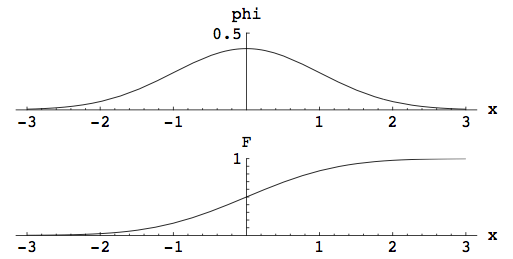
\includegraphics[width=6cm]{./bilder/normalverteilung.png}\\
	Dichtefunktion (oben) und Verteilungsfunktion (unten) der
	Normalverteilung.
\end{minipage}
\hrule

\subsubsection{Standardisierung}
\begin{multicols}{2}
	Erwartungswert: $E(X)=\mu$ \hspace{4mm}(=0 bei Standardnormalver.)\\ 
	Varianz \hspace{11.5mm}: $var(X)=\sigma^2$ (=1 bei Standardnormalver.)\\
	
	$F_Z(z) = P(Z \leq z) = F_X(\sigma z + \mu)$ \\
	$F_X(x) = F_Z(\frac{x-\mu}{\sigma})$\\
	$\varphi_Z(z) = \sigma \cdot \varphi_X(\sigma z + \mu)$\\
	$\varphi_X(x) = \frac{1}{\sigma} \cdot \varphi_Z(\frac{x - \mu}{\sigma})$ 
	\columnbreak

	\fbox{$Z=\dfrac{X-\mu}{\sigma}$} \hspace{5mm} mit $E(Z) = 0$ und $var(Z) = 1$\\ \\
	
	$68\% $ der Werte liegen im Intervall $[ \mu - \sigma, \mu + \sigma]$ \\ 
	$95\% $ in $[ \mu - 2\sigma, \mu + 2\sigma]$ \\
	$99.7\% $ in $[ \mu - 3\sigma, \mu + 3\sigma]$

\end{multicols}

\begin{multicols}{2}
	\textbf{Rezept:} (Berechnen der W'keit das $X\in[x_{min}, x_{max}]$ )
	\begin{enumerate}
		\item W'keit Formel hinschreiben\\
		$P(x_{min} \leq X \leq x_{max})$
		\item Standardisieren:\\
		$P_Z\left(\dfrac{x_{min}-\mu}{\sigma} \leq Z \leq \dfrac{x_{max}-\mu}{\sigma}\right)$
		\item In Verteilungsfunktion einfüllen:\\
		$P_Z=F\left(\dfrac{x_{max}-\mu}{\sigma}\right) - F\left(\dfrac{x_{min}-\mu}{\sigma}\right)$
		\item Werte aus der Tabelle auf Seite \pageref{tbl_NormVerteilung} auslesen:\\
		\textbf{Bei negativen Werten:}\\
		 $F(-0.7) = 1-F(0.7) = 1-0.7580=0.2420$\\[2pt]
		Ist der gesuchte Wert \textbf{zwischen zwei Werten} der Tabelle, dann der Wert aus den benachbarten Werten abschätzen. Bsp:\\ 
		\small 
		$F(0.72) = 0.7642, \quad F(0.73) = 0.7673 \rightarrow F(0.725) \approx 0.765$
		\normalsize
		
	\end{enumerate}
	\columnbreak
	
	\textbf{Beispiel:}\\
	Ein Signal mit normalverteilten Werten $X$ mit Erwartungswert $1$ und Standardabweichung $2$ wird über einen Eingangsverstärker geleitet, der Werte zwischen $\pm 3.3$ verarbeiten kann, bevor er übersteuert wird. Wie häufig wird der Verstärker übersteuert?\\
	$\mu = 1$, $\sigma = 2$
	\begin{enumerate}
		\item $P(-3.3 \leq X \leq 3.3)$
		\item $P\left( \dfrac{-3.3-\mu}{\sigma}
		\leq \dfrac{X-\mu}{\sigma} 
		\leq \dfrac{3.3-\mu}{\sigma} \right)$\\
		$P\left( \dfrac{-3.3-1}{2} \leq Z \leq \dfrac{3.3-1}{2}\right)$\\
		$P(-2.15 \leq Z \leq 1.15)$
		\item $F(1.15) - F(-2.15) = F(1.15) - 1 + F(2.15)$
		\item $0.8749 + 0.9842 - 1 = 0.8591$
	\end{enumerate}
	
\end{multicols}

\hrule
	
\subsubsection{Zentraler Grenzwertsatz}
$X_1, X_2, \ldots , X_n$ sind lauter identisch verteilte (nicht notwendig normalverteilt!)
unabhängige Zufallsvariablen mit demselben Erwartungswert $\mu$ und derselben Varianz $\sigma^2$
und mit $Z = \frac{X-\mu}{\sigma}$. Dann hat die Summe
\begin{equation}
	S_n = \frac{1}{\sqrt{n}}\sum_{i=1}^n Z_i \nonumber
\end{equation}
den Erwartungswert $n \mu$ und die Varianz $n \sigma^2$.\\
Die damit verbundene standardisierte ($E(S_n) = 0, var(S_n) = 1$) Variable $S_n$ ist somit wie
folgt definiert: \\ 
\begin{equation}
	S_n = \frac{1}{\sqrt{n}}\sum_{i=1}^n \frac{X_i - \mu}{\sigma}
	= \frac{1}{\sqrt{n}\cdot \sigma}\left[\left(\sum\limits_{i=1}^n X_i\right) -n \mu\right]
	=\dfrac{\bar{X} - \mu}{\sigma / \sqrt{n}} \nonumber
\end{equation}
Für $\boldsymbol{n \to \infty}$ strebt die Verteilung von $S_n$ gegen die
Standardnormalverteilung. \\


\subsection{Exponentialverteilung}

\begin{minipage}{0.6\textwidth}
	Zur Ermittlung der Dauer bis zum Ausfall/Zerfall von Bauteilen/Stoffen ohne Gedächnis\\
	(W'keit, dass X in der nächsten Minute defekt geht = const.).\\
	Beispiele :
	\begin{itemize}
		\item Lebensdauer von Atomen beim radioaktiven Zerfall
		\item Lebensdauer von Bauteilen, Maschinen \& Geräten\\(MTBF -
		Mean Time Between Failure = $\frac{1}{a}$)
	\end{itemize}
	
	gilt $P(X \leq t) = P(X \leq t_0 + t | X > t_0)$\\
	$P(X > t) = P(X > t_0 + t | X > t_0)$\\
	
	
\end{minipage} \hspace{0.05\textwidth}
\begin{minipage}{0.35\textwidth}
	%Autor: Simon Walker
%Version: 1.0
%Datum: 11.12.2019
%Lizenz: CC BY-NC-SA

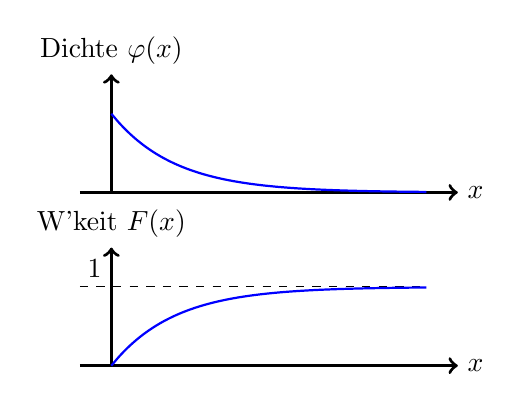
\begin{tikzpicture}[xscale=0.8, yscale=1]
	\def\a{1}
	\def\yOf{2.2} %Y Offsent
	\def\xMax{5}
	
	%Dichte funktion
	%Achsen
	\draw[very thick, ->] (-0.5, \yOf) -- (\xMax+0.5, \yOf);
	\node[right] at (\xMax+0.5, \yOf) {$x$};
	\draw[very thick, ->] (0, \yOf) -- (0, \yOf + \a +0.5);
	\node[above] at (0, \yOf + \a +0.5) {Dichte $\varphi(x)$};
	
	\draw[blue, thick]
	plot[smooth, samples=50, variable=\x, domain=0:\xMax]
	(\x, {\a * exp(\a*\x*-1)+\yOf});
	
	%Verteilungsfunktion
	%Achsen
	\draw[very thick, ->] (-0.5, 0) -- (\xMax+0.5, 0);
	\node[right] at (\xMax+0.5, 0) {$x$};
	\draw[very thick, ->] (0, 0) -- (0, 1.5);
	\node[above] at (0, 1.5) {W'keit $F(x)$};
	
	\draw[dashed] (-0.5, 1) -- (\xMax, 1);
	\node[above left] at (0, 1) {$1$};
	
	\draw[blue, thick]
	plot[smooth, samples=50, variable=\x, domain=0:\xMax]
	(\x, {1- (exp(\a*\x*-1))});
	
\end{tikzpicture}
\\
	Dichtefunktion (oben) und Verteilungsfunktion (unten) der
	Exponentialverteilung.
\end{minipage}

\underline{Dichtefunktion und Verteilungsfunktion}\\
\begin{minipage}{5cm}
	$\varphi(x)=\begin{cases}
	a e^{-a x}  & x \geq 0\\
	0						& x < 0
	\end{cases}$
	
	$F(x)=\begin{cases}
	1-e^{-a x}  		& x \geq 0\\
	0	 					& x < 0
	\end{cases}$
\end{minipage} 
\begin{minipage}{4.5cm}
	$X < x$ Ausfall/Zerfall\\
	$X > x$ kein Ausfall/Zerfall
\end{minipage}\\
    
\begin{minipage}[t]{6cm}
  \underline{Erwartungswert und Varianz}\\[4pt]
  $E(X)=\dfrac{1}{a}$\\
  $var(X)=\dfrac{1}{a^2}$ 
\end{minipage}
\begin{minipage}[t]{9cm}
  \underline{Lebensdauer von mehreren \textbf{unabhängigen} Bauteilen}
  \begin{align}
    P(X>x) &= P(X_1>x_1 \cap X_2>x_2 \cap X_3>x_3 \ldots) \nonumber \\
    &= P(X_1>x_1) \cdot P(X_2>x_2) \cdot P(X_3>x_3) \ldots \nonumber \\
    &= (1-P(X_1\leq x_1)) \cdot (1-P(X_2\leq x_2)) \cdot (1-P(X_3\leq x_3)) \ldots \nonumber \\
    &= (1-F(x_1)) \cdot (1-F(x_2)) \cdot (1-F(x_3)) \ldots \nonumber
  \end{align}
\end{minipage}
		
	\hrule

\subsection{Hypergeometrische Verteilung}

      	
\begin{minipage}{0.7\textwidth}
	Ist die Wahrscheinlichkeit dass in einer $m$ Elemente umfassenden 
	Stichprobe aus einer Grundgesamtheit von $n$ Elementen, von denen $r$ eine
	spezielle Eigenschaft besitzen, $k$ Elemente mit der Eigenschaft zu
	finden sind.\\
	\vspace{5mm} 
	$p(k)=P(X=k)=\dfrac{\binom r k \binom{n-r}{m-k}}{\binom n m}$ 
	\hspace{10mm} für $0\leq k \leq r$ und $k \leq n$\\
	Erwartungswert: \hspace{10mm} $E(X)=m \dfrac{r}{n}$\\
	Varianz: \hspace{22mm} $var(X)=m \dfrac{r(n-r)(n-m)}{n^2(n-1)}$ \\
	{\bf Beispiel:} \\
	Lotto, $n=45$ Zahlen, $r=6$ (die gezogenen Zahlen), $m=6$
	(meine Zahlen) \\
	$P(X=4)=P(\text{Ein Vierer})=\dfrac{\binom 6 4 \binom {39}
	2}{\binom {45} 6}=0.001364$
\end{minipage}
\begin{minipage}{0.3\textwidth}
	%Autor: Simon Walker
%Version: 1.0
%Datum: 11.12.2019
%Lizenz: CC BY-NC-SA

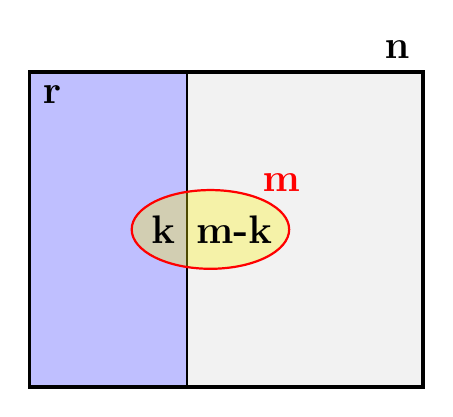
\begin{tikzpicture}
%	\newcommand{\HelpCords}[4]{
%		\draw [help lines] (#1,#2) grid (#3,#4);
%		\foreach \i in {#1,..., #3}
%		\node [below] at (\i,#2) {$\i$};
%		\foreach \i in {#2,..., #4}
%		\node [left] at (#1,\i) {$\i$};
%	}
	
	\filldraw[thick, draw=black, fill=blue!25] (0, 0) rectangle (2, 4);
	\filldraw[thick, draw=black, fill=gray!10] (2, 0) rectangle (5, 4);
	
	\filldraw[thick, draw=red, fill=yellow, fill opacity=.3]
	(2.3, 2) ellipse (1 and 0.5);	
	
	\draw[very thick] (0, 0) rectangle (5, 4);
	
	\Large
	\node[below right] at (0, 4) {\textbf{r}};
	\node[above left] at (5, 4) {\textbf{n}};
	\node at (1.7, 2) {\textbf{k}};
	\node at (2.6, 2) {\textbf{m-k}};
	\node[red] at (3.2, 2.6) {\textbf{m}};
	
	\normalsize
	
%	\HelpCords{0}{0}{5}{4}
\end{tikzpicture}

\end{minipage}


\hrule \hspace{3mm}

	\subsection{Poissonverteilung \skript{\pageref{sk-section-poissonverteilung}}}
	\begin{multicols}{2}
		\begin{tabular}{ll}
        $P_\lambda(k)=\frac{\lambda^k}{k!}e^{-\lambda}$ &
         \parbox{4cm}{W'keit dass k Ereignisse im Intervall [0,x] auftreten} \\
        Erwartungswert:  & $E(X)=\lambda$\\
        Varianz:  & $var(X)=\lambda$ \\
        %$\lambda = a \cdot x$ \\
        \end{tabular} \\
         $P(X<k) \leq \sum_0^k P_\lambda(k)=\sum_0^k \frac{\lambda^k}{k!}e^{-\lambda}$ \\
         $P(X>k) = 1-P(X<k)$ \\
        $x =$ Anzahl Versuche\\
        $\lambda =$ Ereignisse pro Intervall im Mittel
        \columnbreak
        
        {\bf Anwendungsbeispiele:} \\ Für die Häufigkeiten seltener
        Ereignisse. Anzahl Anrufe bei einer Telefonzentrale in einer gewissen
        Periode. Anzahl grosse Versicherungsschäden in einer gewissen Periode.
        Anzahl Jobs, die bei einem Server ankommen. Anzahl Ereignisse in
        einem Zeitintervall. Anzahl Lokomotiven der SBB, die in der nächsten Woche 
        einen Defekt haben. Anzahl der Gewinner mit 4 Richtigen im Lotto.
     \end{multicols}
        
\hrule
	\subsection{Binomialverteilung \skript{\pageref{sk-section-binomialverteilung}}}
		
    	Wird angewendet bei einem Experiment mit nur zwei Ausgängen (Ereignis mit W'keit $p$ tritt
    	ein, Ereignis tritt nicht ein). \\
    	Eine Zufallsvariable mit diskreten Werten $k \in \{
    	0,\ldots,n \}$ heisst binomialverteilt zum Parameter $p$, wenn die
        Wahrscheinlichkeit des Wertes $k$ wie folgt ist:

      $$P(X=k) = \binom n k p^k(1-p)^{n-k} \qquad \mu = E(X) = p \cdot n \qquad \sigma^2 =
      var(X) = n \cdot p (1-p)$$

      $n$: Versuche \hspace{10mm}
      $k$: k-mal erfolgreich \hspace{10mm}
      $p$: Wahrscheinlichkeit\\
      
      Approximation mit Normalverteilung: $P(a \leq x \leq b) \simeq \underbrace{P(a-0.5 \leq x \leq b+0.5)}_{\text{Normalverteilung}}$\\
      
      {\bf Beispiel:} Wie hoch ist die Wahrscheinlichkeit, dass bei 350 Leuten genau
      k $(k\leq 350)$ heute Geburtstag haben?\\
      $P(k)=\binom {350} k \left(\frac{1}{365}\right)^k
      \left(\frac{364}{365}\right)^{350-k}$ \\



\hrule
		\subsection{Gleichverteilung}
      \begin{multicols}{3}
        \textbf{Stetig \skript{\pageref{sk-section-gleichverteilung-stetig}}}\\ \\
        $\varphi(x) = \begin{cases}
          0 & x < a\\
          \frac{1}{b-a} & x \in [a, b]\\
          0 & x > b
        \end{cases}$ \\
        $F(x) = \begin{cases}
          0 & x < a\\
          \frac{x-a}{b-a} & x \in [a,b]\\
          1 & x > b
        \end{cases}$\\
        \begin{tabular}{ll}
          Erwartungswert: & $E(X)=\frac{a + b}{2}$\\
          Varianz:  &$var(X)=\frac{(b-a)^2}{12}$\\
        \end{tabular}
      \columnbreak
      
        \textbf{Diskret \skript{\pageref{sk-section-gleichverteilung-diskret}}}\\ \\
        $F(x) = \begin{cases}
          0 & x \leq 1\\
          \frac{|x|}{n} & 1 \leq x \leq n \\
          1 & x \geq n
        \end{cases}$\\
        \begin{tabular}{ll}
          Wahrscheinlichkeit: & $p(k) = \frac{1}{n}$\\
          Erwartungswert: & $E(X)=\frac{n + 1}{2}$\\
          Varianz: & $var(X)=\frac{n^2-1}{12}$\\
          $E(X^2) = \frac{2n^2+3n+1}{6}$ &
        \end{tabular}
      \columnbreak
      	%Autor: Simon Walker
%Version: 1.0
%Datum: 13.12.2019
%Lizenz: CC BY-NC-SA

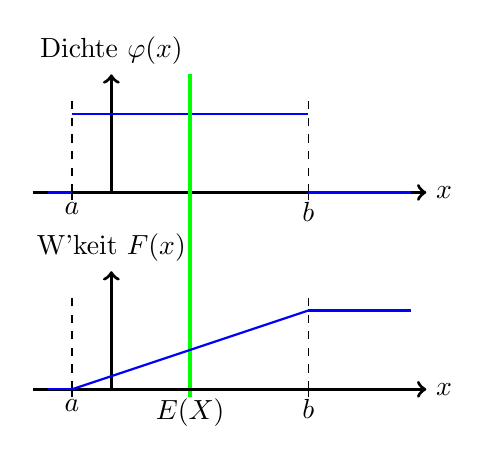
\begin{tikzpicture}
	\newcommand{\HelpCords}[4]{
		\draw [help lines] (#1,#2) grid (#3,#4);
		\foreach \i in {#1,..., #3}
		\node [below] at (\i,#2) {$\i$};
		\foreach \i in {#2,..., #4}
		\node [left] at (#1,\i) {$\i$};
	}

	\def\yOf{2.5}
	\def\a{-0.5}
	\def\b{2.5}
	\def\EWert{{(\a+\b)/2}}
	
	%Dichte funktion
	%Achsen
	\draw[very thick, ->] (-1, \yOf) -- (4, \yOf);
	\node[right] at (4, \yOf) {$x$};
	\draw[very thick, ->] (0, \yOf) -- (0, \yOf + 1.5);
	\node[above] at (0, \yOf + 1.5) {Dichte $\varphi(x)$};
	
	\draw (\a, -0.1+\yOf) -- (\a, +0.1+\yOf);
	\node[below] at (\a, \yOf) {$a$};
	\draw[dashed] (\a, \yOf) -- (\a, \yOf + 1.2);
	\draw (\b, -0.1+\yOf) -- (\b, +0.1+\yOf);
	\node[below] at (\b, \yOf) {$b$};
	\draw[dashed] (\b, \yOf) -- (\b, \yOf + 1.2);
	
	%Funktion
	\draw[blue, thick] (-0.8, \yOf) -- (\a, \yOf);
	\draw[blue, thick] (\a, \yOf + 1) -- (\b, \yOf +1);
	\draw[blue, thick] (\b, \yOf) -- (3.8, \yOf);
	
	
	%Erwartungswert
	\draw[green, very thick] (\EWert, -0.1) -- (\EWert, 1.5 + \yOf);
	\node[below] at (\EWert, 0) {$E(X)$};

	
	
	
	%Verteilungsfunktion
	%Achsen
	\draw[very thick, ->] (-1, 0) -- (4, 0);
	\node[right] at (4,0) {$x$};
	\draw[very thick, ->] (0, 0) -- (0, 1.5);
	\node[above] at (0, 1.5) {W'keit $F(x)$};
	
	\draw (\a, -0.1) -- (\a, +0.1);
	\node[below] at (\a, 0) {$a$};
	\draw[dashed] (\a, 0) -- (\a, 1.2);
	\draw (\b, -0.1) -- (\b, +0.1);
	\node[below] at (\b, 0) {$b$};
	\draw[dashed] (\b, 0) -- (\b, 1.2);
	
	%Funktion
	\draw[blue, thick] (-0.8, 0) -- (\a, 0);
	\draw[blue, thick] (\a, 0) -- (\b, 1);
	\draw[blue, thick] (\b, 1) -- (3.8, 1);
	
	
	%\HelpCords{-1}{0}{4}{5}
\end{tikzpicture}
\\ 
        Stetig: Blau \quad Diskret: Braun
      \end{multicols}
  
  \hrule 
      
	\subsection{Potenzgesetze (Power-Laws) \skript{\pageref{sk-potenzgesetze}}}
	Die Normalverteilung beschreibt (physikalische) Grössen, die vor allem in einer bestimmten
	Grössenordnung vorkommen. Die Potenzgesetze dienen dazu, Grössen welche einen grossen
	Wertebereich annehmen können, zu beschreiben.
	
    \begin{multicols}{2}
		$\varphi(x) = \begin{cases}
		\frac{\alpha - 1}{x_{min}^{1-\alpha}}\cdot x^{-\alpha} & x > x_{min} \\
		0 & sonst
		\end{cases} \qquad $ mit $\alpha > 1$\\
		
    \columnbreak
    
		$E(X) = \frac{\alpha - 1}{\alpha - 2} \cdot x_{min}$ \\
		$E(X^2) = \frac{\alpha - 1}{\alpha - 3} \cdot x_{min}^2$ \\
 		$var(X) = \left(\frac{\alpha - 1}{\alpha - 3} - \left(\frac{\alpha -1}{\alpha -2}\right)^2\right)\cdot x_{min}^2$ \\
 		$x_{\frac{1}{2}} = 2^{\frac{1}{\alpha - 1}} \cdot x_{min}$ \\
	\end{multicols}
	
	Eine nach dem Potenzgesetz verteilte Zufallsvariable kann man daran erkennen, dass die Dichtefunktion in doppelt logarithmischer Darstellung eine Gerade ist. Wegen
	$\log p(x) = -\alpha \log x + \log C$ ist die Steigung der Geraden $-\alpha$. \\
	
	Der Parameter $\alpha$ kann mithilfe eines Maximum-Likelihood Schätzers bestimmt werden. Es gilt: $\alpha = 1 + \frac{n}{\sum_{i=1}^{n}} \log \frac{x_i}{x_min}$ \\
\hrule
